\documentclass[conference]{IEEEtran}
\usepackage{cite}
\usepackage{graphicx}
\usepackage{booktabs}
\usepackage{url}
\usepackage{amsmath}
\usepackage{placeins}
\title{Software Defect Prediction Across 20 Datasets: An Empirical Comparison of Ten Classifiers}
\author{\IEEEauthorblockN{Aditya Dubey}}
\begin{document}
\maketitle
\begin{abstract}
Software defect datasets are imbalanced, and accuracy can conceal weak detection of defective modules. We compare ten supervised classifiers across 20 larger datasets from the DefectData repository using three grouped stratified folds per dataset. Methods include Decision Tree, K-nearest neighbors, XGBoost, Random Forest, Linear SVM, Logistic Regression, PCA plus Logistic Regression, AdaBoost, a multilayer perceptron, and Gaussian Naive Bayes. We report accuracy, precision, recall, F1, Matthews correlation coefficient (MCC), and ROC-AUC. Equal-weight macro averages show that XGBoost achieved the highest ROC-AUC (0.798), F1 (0.485), and MCC (0.371); Random Forest had the highest accuracy (0.837) and precision (0.511); AdaBoost had the highest recall (0.691). A majority-class baseline achieved 0.812 accuracy but zero defect recall. Results are descriptive; no hyperparameter search or significance test was performed.
\end{abstract}
\begin{IEEEkeywords}
software defect prediction, classification, cross-dataset evaluation, XGBoost, MCC, ROC-AUC
\end{IEEEkeywords}
\section{Introduction}
Software defect prediction estimates whether a software module is defective from code metrics. It can support review prioritization, but defect labels are commonly imbalanced and false negatives may be costly. Accuracy alone is inadequate; evaluation should include minority-class measures and ranking metrics \cite{menzies2007,kamei2013}.

We extend earlier JM1 and PROP-1 experiments to a 20-dataset comparison and add seven algorithms to the original Decision Tree, KNN, and XGBoost set. We ask how these ten methods compare on defect identification and ranking across larger public data.

Each model is trained and evaluated separately on each dataset because feature definitions vary across corpora. We examine whether the model with the best average ranking also leads on individual datasets, and whether reducing the input dimension with PCA improves Logistic Regression. The evaluation estimates performance on held-out modules from the same dataset.
\section{Data and Preparation}
Data were obtained from the DefectData repository \cite{defectdata}. Datasets were eligible when they contained at least 50 defective and 50 non-defective records; the 20 largest eligible datasets by row count were selected: prop-1, prop-2, prop-3, prop-4, prop-5, JM1, PC3, PC4, PC5, eclipse-2.0, eclipse-2.1, eclipse-3.0, eclipse34\_debug, eclipse34\_swt, mylyn, pde, jdt, camel-1.4, camel-1.6, and xalan-2.6. Together they contain 115,688 records and 16,659 defects. Source-specific target definitions were retained, while identifiers and targets were excluded from predictors.

Numeric predictors were retained, and wholly missing features were removed. No selected dataset had missing feature cells; median imputation remained in pipelines as a safeguard. Scaling was used for distance, linear, and neural methods. Imbalance handling was model-specific. Three stratified grouped folds (seed 42) were applied per dataset, keeping identical feature vectors together where group class support allowed.

Dataset sizes range from 872 to 23,014 records, with 15 to 38 features. Positive labels account for 14.4\% of all rows pooled across datasets. Count-based targets were converted to binary labels by marking any positive defect count as defective. All 20 datasets used grouped splits. For example, PROP-2 contains 23,014 rows with 12,649 distinct predictor vectors. Grouping keeps each repeated pattern on one side of a split. Table~\ref{tab:datasets} gives the complete inventory and the top ROC-AUC on each dataset.
\section{Methods}
The ten algorithms below were selected to compare interpretable rules, distance-based classification, linear margins, probabilistic models, ensembles, and a neural network. All configurations were fixed before scoring the held-out folds.
\subsection{Decision Tree}
A Decision Tree recursively selects a metric and threshold to make resulting groups more class-pure. Trees capture nonlinear rules without scaling and are relatively easy to inspect. We used Gini splitting, maximum depth 6, minimum leaf size 10, and balanced class weights so minority-class errors receive greater influence.
\subsection{K-Nearest Neighbors}
KNN assigns a module the majority label among its closest training examples. The five-neighbor model used Euclidean distance after standard scaling; otherwise metrics with larger numeric ranges could dominate the distance. KNN can model local nonlinear boundaries, but may be sensitive to redundant or noisy variables.
\subsection{XGBoost}
XGBoost constructs boosted decision trees sequentially, with each new tree reducing the residual loss while regularization controls model complexity \cite{chen2016}. The configuration used 120 trees, depth 4, learning rate 0.05, row and feature subsampling of 0.8, and L2 regularization of 1. The positive-class weight was set to the negative-to-positive ratio in the training fold.
\subsection{Random Forest}
Random Forest trains trees on bootstrap samples and random predictor subsets, then combines their votes. Averaging reduces the variance of a single tree and captures nonlinear feature interactions. We used 120 trees, minimum leaf size 2, and balanced class weighting within each bootstrap sample.
\subsection{Linear SVM}
A linear Support Vector Machine selects a separating hyperplane with a wide margin between classes. Its signed decision score indicates distance from the boundary. Predictors were standardized, class weights were balanced, and $C=1$. Labels use the zero-score boundary; continuous scores are retained for ROC-AUC.
\subsection{Logistic Regression}
Logistic Regression applies a sigmoid to a weighted sum of metrics to estimate defect probability. It gives a linear decision boundary and probability scores, but correlated metrics can make individual coefficients unstable. We standardized inputs, used balanced class weights and the liblinear solver, and allowed up to 1,500 iterations.
\subsection{PCA and Logistic Regression}
Principal Component Analysis (PCA) rotates standardized metrics into orthogonal directions ranked by explained variance. The pipeline retained enough components to explain 95\% of variance, then fit class-balanced Logistic Regression. PCA was fitted inside each training fold to avoid using test data during dimensionality reduction.
\subsection{AdaBoost}
AdaBoost combines weak learners in sequence, increasing the influence of examples misclassified by earlier learners. Its final score is a weighted combination of learner outputs. The experiment used 80 decision stumps (depth-one trees), learning rate 0.5, and balanced sample weights.
\subsection{Neural Network}
The Multilayer Perceptron (MLP) learns nonlinear metric interactions through connected layers and ReLU activations. It used two hidden layers with 32 and 16 units, L2 penalty 0.001, batch size 256, and early stopping. Predictors were standardized and training examples resampled to balance the classes. The 55-iteration cap was reached in some folds, so the MLP is a fixed-budget baseline.
\subsection{Gaussian Naive Bayes}
Gaussian Naive Bayes applies Bayes' rule under conditional independence of predictors within each class and a Gaussian distribution for each metric. It combines metric-wise likelihoods into a class posterior. We standardized inputs, set equal class priors, and used variance smoothing of $10^{-8}$.
\subsection{Evaluation}
CNN was excluded because the inputs are flat metric vectors without spatial structure; Gaussian Mixture was excluded because the task is supervised binary classification. We report accuracy, defect-class precision, recall, F1, Matthews correlation coefficient (MCC), and ROC-AUC. Hard-label metrics use a fixed probability threshold of 0.5; Linear SVM uses its zero decision boundary. ROC-AUC uses continuous model scores \cite{fawcett2006}. Fold metrics were averaged per dataset, then the 20 dataset means were averaged equally. A majority-class model predicting every module non-defective provides an accuracy baseline.
Across the 20 datasets, the protocol produced 600 held-out model evaluations. With defective modules as the positive class, precision is the fraction of flagged modules that are defective, and recall is the fraction of all defective modules flagged. F1 and MCC use the confusion counts $TP$, $FP$, $FN$, and $TN$:
\begin{align}
F_1 &= \frac{2TP}{2TP+FP+FN},\\
\mathrm{MCC} &= \frac{TP\,TN-FP\,FN}{\sqrt{D}},\\
D &= (TP+FP)(TP+FN)(TN+FP)(TN+FN).
\end{align}
MCC ranges from $-1$ to $1$. Accuracy counts correctly classified modules of both classes. ROC-AUC measures how well the scores rank defective modules above non-defective ones across thresholds.
\section{Results}
Table~\ref{tab:results} presents the macro averages. XGBoost led in ROC-AUC (0.798), F1 (0.485), and MCC (0.371). Random Forest reached the highest accuracy (0.837) and precision (0.511). AdaBoost had the highest recall (0.691). The majority baseline had 0.812 accuracy with zero recall for defects, illustrating the limitation of accuracy under class imbalance.

Figure~\ref{fig:box} shows the spread of dataset means. In Fig.~\ref{fig:auc}, XGBoost led on 12 datasets and Random Forest led on six. Linear SVM led on camel-1.4, and Logistic Regression led on mylyn.
\begin{table*}[t]
\caption{Equal-weight macro averages across 20 datasets (three folds per dataset)}
\label{tab:results}\centering\footnotesize
\begin{tabular}{lrrrrrr}\toprule
Model & Accuracy & Precision & Recall & F1 & MCC & ROC-AUC\\\midrule
XGBoost & 0.773 & 0.412 & 0.637 & 0.485 & 0.371 & 0.798\\
Random Forest & 0.837 & 0.511 & 0.366 & 0.413 & 0.332 & 0.791\\
AdaBoost & 0.707 & 0.354 & 0.691 & 0.448 & 0.322 & 0.773\\
Logistic Regression & 0.727 & 0.368 & 0.645 & 0.448 & 0.321 & 0.764\\
Linear SVM & 0.728 & 0.369 & 0.642 & 0.448 & 0.321 & 0.763\\
Neural Network (MLP) & 0.719 & 0.356 & 0.644 & 0.439 & 0.307 & 0.759\\
PCA + Logistic Regression & 0.726 & 0.364 & 0.634 & 0.443 & 0.312 & 0.758\\
Decision Tree & 0.708 & 0.347 & 0.677 & 0.444 & 0.311 & 0.740\\
Gaussian Naive Bayes & 0.757 & 0.435 & 0.362 & 0.346 & 0.249 & 0.723\\
KNN ($k=5$) & 0.833 & 0.475 & 0.275 & 0.338 & 0.264 & 0.723\\\bottomrule
\end{tabular}
\end{table*}
\begin{table}[t]
\caption{Dataset Sizes, Defect Counts, and Best ROC-AUC}
\label{tab:datasets}\centering\footnotesize
\begin{tabular}{lrrlr}
\toprule
Dataset & Rows & Defects & Leader & AUC\\
\midrule
prop-2 & 23,014 & 2,431 & RF & 0.835\\
prop-1 & 18,471 & 2,738 & XGB & 0.792\\
eclipse-3.0 & 10,593 & 1,568 & XGB & 0.808\\
prop-3 & 10,274 & 1,180 & XGB & 0.746\\
prop-4 & 8,718 & 840 & XGB & 0.790\\
prop-5 & 8,516 & 1,299 & XGB & 0.750\\
eclipse-2.1 & 7,888 & 854 & XGB & 0.791\\
JM1 & 7,782 & 1,672 & XGB & 0.696\\
eclipse-2.0 & 6,729 & 975 & XGB & 0.845\\
mylyn & 1,862 & 245 & LR & 0.796\\
PC5 & 1,711 & 471 & XGB & 0.788\\
pde & 1,497 & 209 & XGB & 0.765\\
eclipse34\_swt & 1,485 & 653 & RF & 0.970\\
PC4 & 1,287 & 177 & RF & 0.935\\
PC3 & 1,077 & 134 & RF & 0.829\\
eclipse34\_debug & 1,065 & 263 & XGB & 0.806\\
jdt & 997 & 206 & RF & 0.812\\
camel-1.6 & 965 & 188 & XGB & 0.709\\
xalan-2.6 & 885 & 411 & RF & 0.864\\
camel-1.4 & 872 & 145 & SVM & 0.720\\
\bottomrule
\end{tabular}
\par\smallskip\raggedright
RF = Random Forest. XGB = XGBoost. LR = Logistic Regression.
\end{table}
\begin{figure*}[t]\centering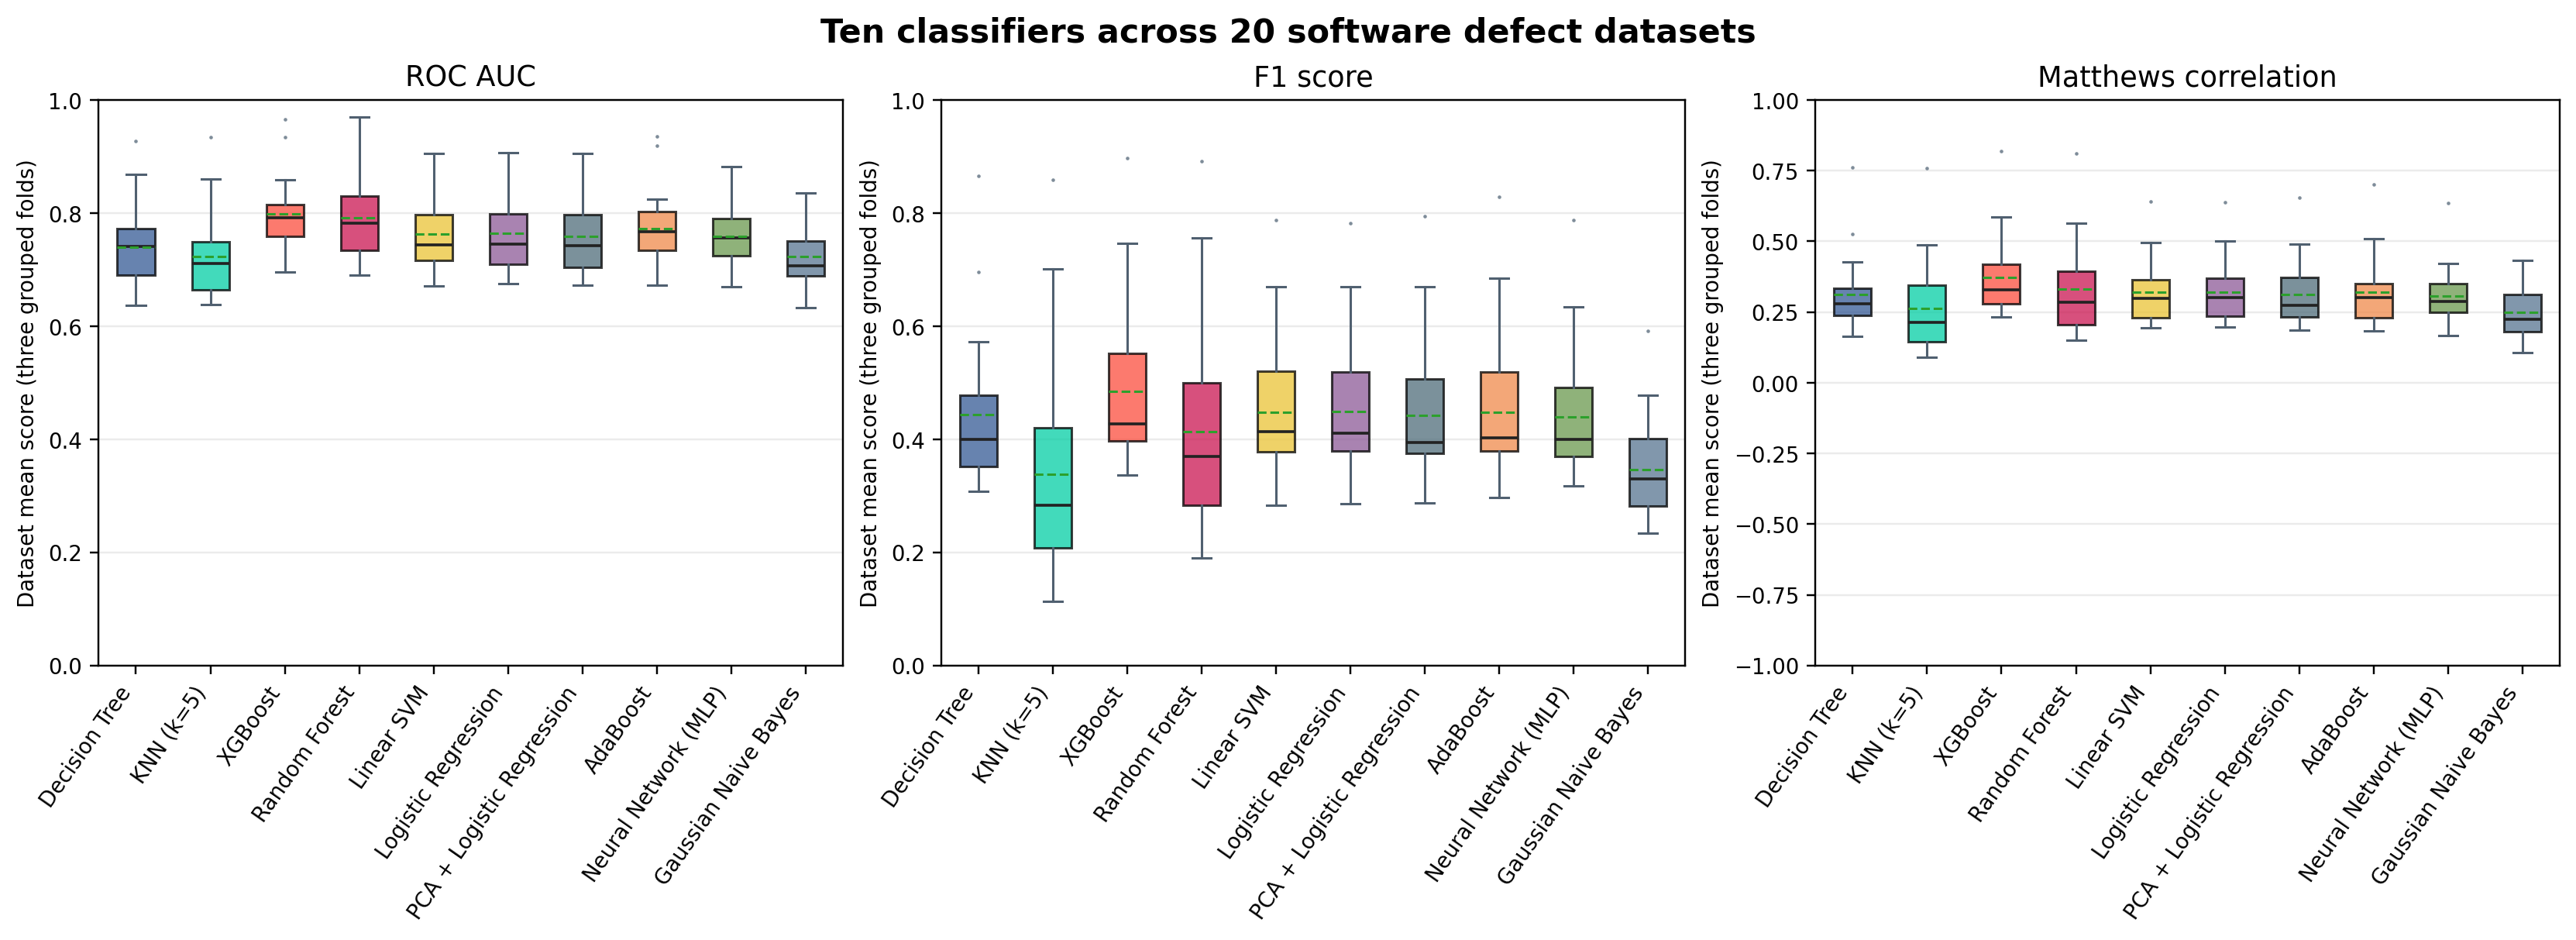
\includegraphics[width=0.78\textwidth]{figures/model_performance_boxplots.png}\caption{Distribution of dataset-level scores across 20 datasets.}\label{fig:box}\end{figure*}
\begin{figure*}[t]\centering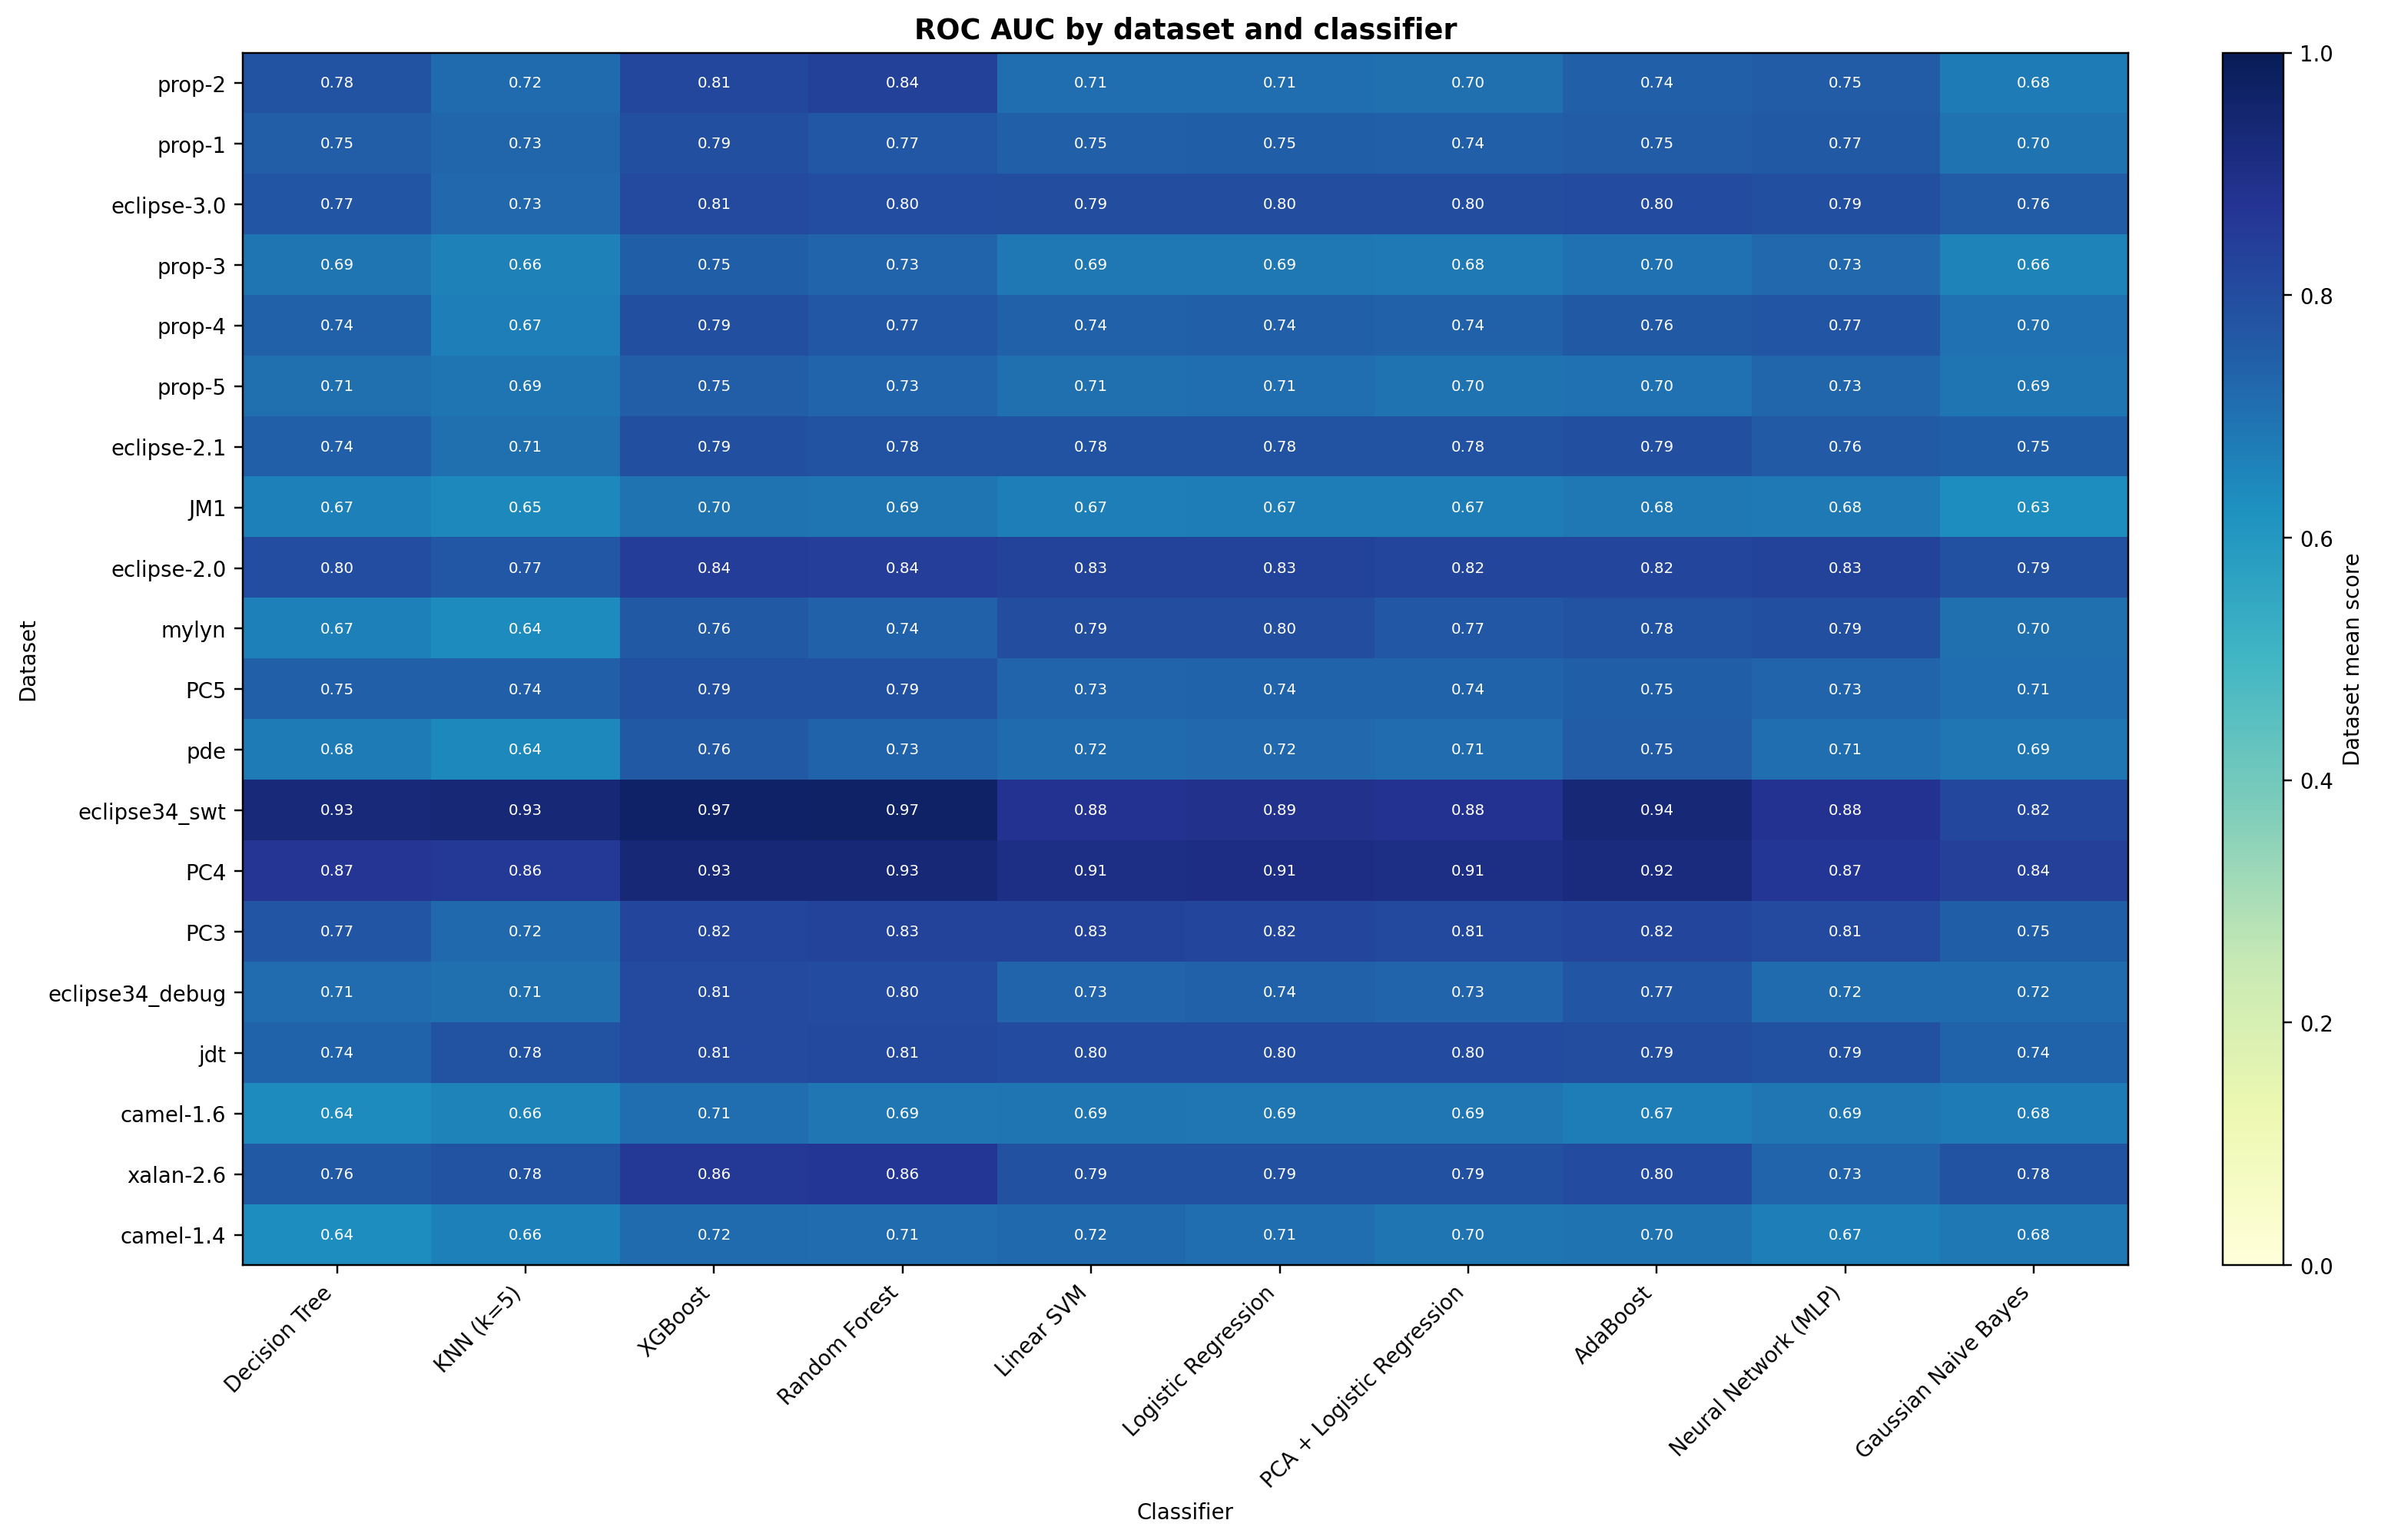
\includegraphics[width=0.82\textwidth]{figures/roc_auc_heatmap.png}\caption{Three-fold ROC-AUC means by dataset and classifier.}\label{fig:auc}\end{figure*}
\begin{figure}[t]\centering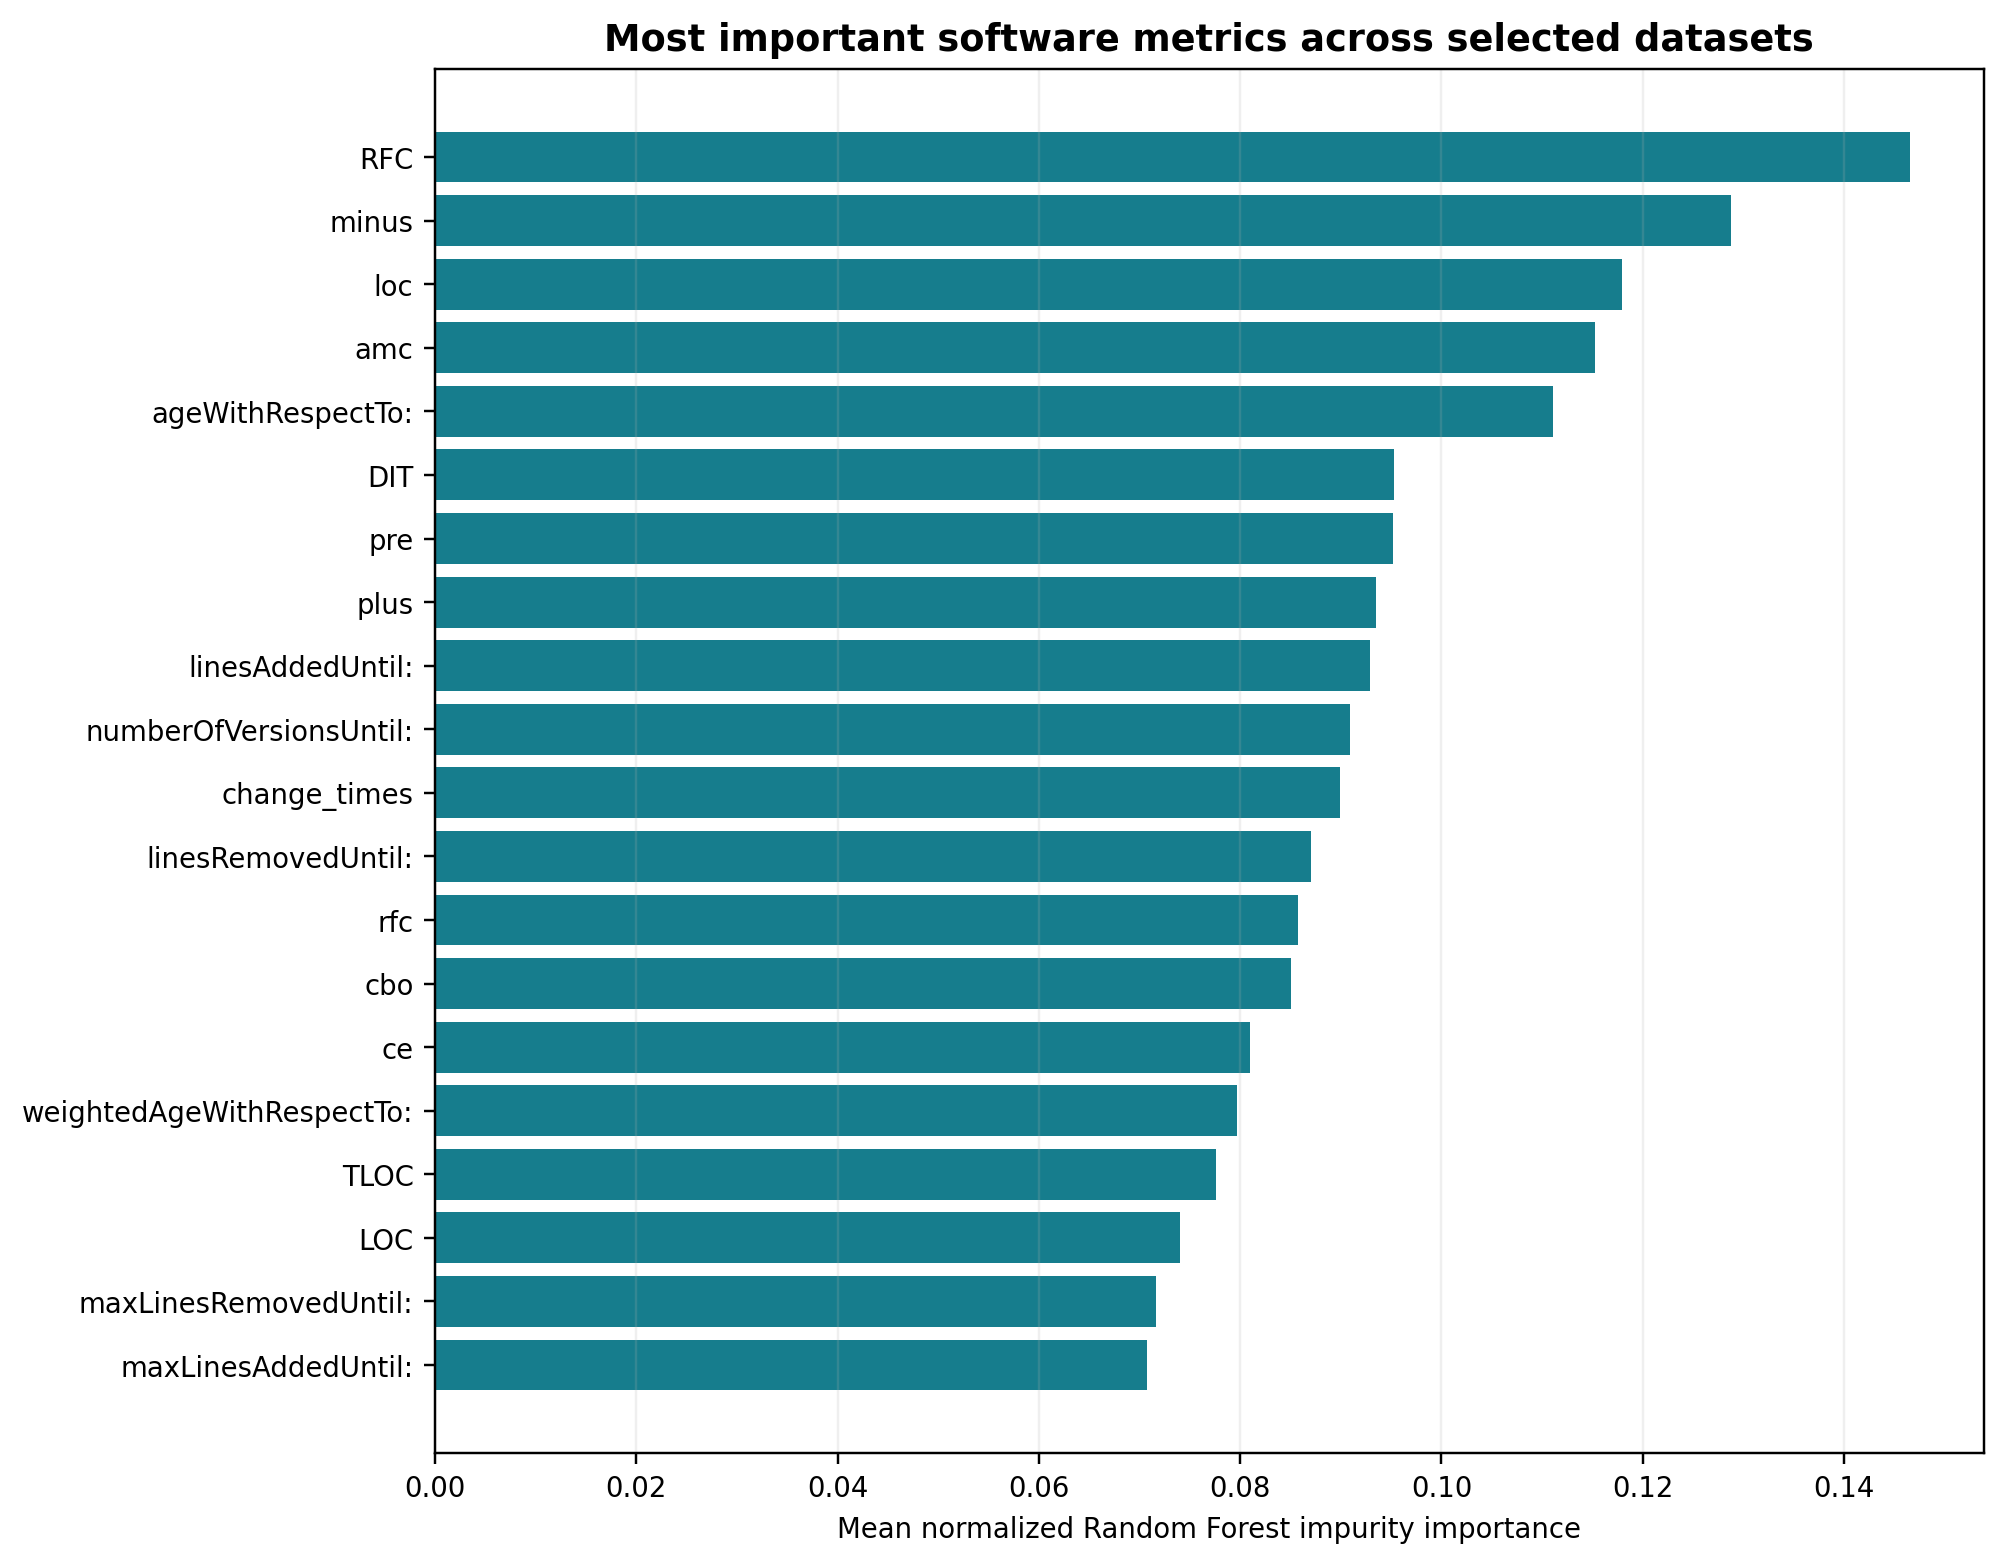
\includegraphics[width=\columnwidth]{figures/random_forest_feature_importance.png}\caption{Leading aggregated Random Forest feature importances.}\label{fig:features}\end{figure}
\FloatBarrier
\section{Discussion}
XGBoost led on JM1 (0.696) and PROP-1 (0.792), while Random Forest reached 0.970 on eclipse34\_swt and 0.935 on PC4. The standard deviations of dataset ROC-AUC were 0.067 for XGBoost and 0.074 for Random Forest. KNN reached 0.833 accuracy but found only 27.5\% of defects on average at its default cutoff.

XGBoost's average ROC-AUC exceeded Random Forest's by about 0.007. The study did not test the statistical significance of this difference. Random Forest gives higher precision at the tested thresholds, so a larger share of the modules it flags are defective. AdaBoost gives higher recall, so it finds a larger share of defects and makes more false alarms. Thresholds should reflect inspection capacity and the costs of each error. A team interested in a fixed review budget could compare precision or lift at the same number of inspected modules.

Adding PCA reduced average ROC-AUC from 0.764 to 0.758 and F1 from 0.448 to 0.443 relative to Logistic Regression. PCA orders components by feature variance, so a direction with low variance can still carry information about defects. The observed score differences do not isolate that mechanism.

Figure~\ref{fig:features} shows mean impurity importance for Random Forest, averaged over fits from datasets in which each named feature appeared. Features occur in different numbers of datasets. Correlated predictors can share split importance, and similar feature names can reflect different measurement definitions. The chart describes how the forests split the available inputs.

The MLP reached its 55-iteration cap in some folds. Its results reflect the architecture and training budget used here. The model configurations also used different weighting or resampling schemes. A study isolating the effect of model architecture would need a common design for weighting and tuning.
\section{Threats to Validity}
This study covers 20 datasets from one repository, fixed configurations, and three folds per dataset. The size and class-count filters favor larger datasets with adequate representation of both classes. Related releases can share project conventions and module histories even when their feature vectors differ. The grouped split addresses exact matches within each dataset. Predictions on future releases or unfamiliar projects would require separate validation, with splits organized by release date or by project.

\section{Conclusion}
Across these data, XGBoost led on macro ROC-AUC, F1, and MCC. Random Forest led on accuracy and precision, and AdaBoost led on recall. The majority-class accuracy of 0.812 and recall of zero show the value of reporting several metrics. A follow-up study could select thresholds using training data, evaluate on independent projects, and quantify paired differences across repeated splits.
\bibliographystyle{IEEEtran}
\bibliography{references}
\end{document}
